\section{Background}
\label{background}

As touched upon in section \ref{introduction}, locality-sensitive hashing tackles the problem of similarity search in high-dimensional datasets by relaxing the requirement of finding exact nearest neighbours. Instead, LSH is used as an \textit{approximate} nearest neighbour algorithm, which inherently implies only probabilistic guarantees of finding a nearest neighbour. In general, LSH schemes act as randomized filters that attempt to reduce an input set to a subset of candidates for a given query item.

The formal definition of the approximate nearest neighbour problem for Hamming space is given as follows in \cite{DBLP:journals/corr/PhamP16}:

\begin{definition}
\label{definition-nearest-neighbour}
  Given a set $S \subset \{0, 1\}^d$, $|S| = n$, the Hamming distance function $D$, and parameters $r > 0$, $c > 1$, $\delta > 0$, construct a data structure such that, given any query $q \in \{0,1\}^d$, if there exists a point $x \in S$ and $D(x, q) \leq r$, it reports some point $y \in S$ where $D(y, q) \leq cr$ with probability $1 - \delta$.
\end{definition}

Here, $\delta$ defines the rate of occurences of false negatives.

The data structure mentioned in definition \ref{definition-nearest-neighbour} makes use of a family of \textit{locality-sensitive hash functions} in order to hash items to buckets. The definition of this family is given as follows in \cite{DBLP:conf/stoc/IndykM98}:

\begin{definition}
\label{definition-hash-functions}
  Given $r$, $c$, $p_1$, $p_2$, and $c > 1$, $p_1 < p_2$, a family $H = \{h \colon S \rightarrow U\}$ is said to be $(r, cr, p_1, p_2)$-sensitive for $(S, D)$ if for any $q,p \in S$ we have

  \begin{itemize}
    \item if $D(p, q) \leq r$ then $Pr_H [h(q) = h(p)] \geq p_1$,
    \item if $D(p, q) > cr$ then $Pr_H [h(q) = h(p)] \leq p_2$.
  \end{itemize}
\end{definition}

Here, $p_1$ is the lower bound on the probablity of close vectors colliding and $p_2$ is the upper bound on the probability of distant vectors colliding \cite[p. 100]{DBLP:books/cu/LeskovecRU14}. As such, we want $p_1$ to be close to 1 whereas we want $p_2$ to be close to 0. The intricate details of these collision probabilities will however not be touched more upon in this paper; we instead refer to \cite{DBLP:conf/stoc/IndykM98} and \cite{DBLP:books/cu/LeskovecRU14}.

\subsection{Classic LSH}
\label{background-classic-lsh}

The classic LSH scheme for Hamming space uses a random bit sampling approach for picking a number of components from an input vector. This sample is then used as the key in a map structure, which will be referred to as a \textit{partition}, for locating a bucket that the vector should be stored in. The bits to sample for a given partition are chosen independently and uniformly at random and stored with the partition. When looking for the nearest neighbour of a query vector, this sampling is repeated and the candidate vectors are those found in the bucket that the sample maps to.

\begin{example}
\label{example-classic-sampling}
Given input vector $v = 1101$, we randomly chose to sample component 1 and 3, giving us the key $v' = 10$. We then proceed to update our map structure with an entry for this key: $10 \rightarrow \{1101\}$

Given another input vector $u = 0110$, we again sample component 1 and 3, giving us the key $u' = 01$. We then add another entry to our map: $10 \rightarrow \{1101\}, 01 \rightarrow \{0110\}$.

Given a query vector $q = 1001$, we once again sample component 1 and 3, giving us the key $q' = 10$. We then look up this key in our map and receive the following set of candidates: $\{1101\}$.
\end{example}

\begin{figure}[ht]
  \centering
  \begin{tikzpicture}
    \node (u) {u = \underline{0}1\underline{1}0};
    \node (v) [right=of u] {v = \underline{1}1\underline{0}1};
    \node (q) [right=of v] {q = \underline{1}0\underline{0}1};

    \matrix (m) [matrix of nodes, below=of v, row sep=-\pgflinewidth, style={nodes={draw}}]{
    01 & 10 & 11 \\
    };

    \path [->] (u.south) edge ([yshift=0.5ex] m-1-1.north);
    \path [->] (v.south) edge ([yshift=0.5ex] m-1-2.north);
    \path [->] (q.south) edge ([yshift=0.5ex, xshift=0.5ex] m-1-2.north);
  \end{tikzpicture}

  \caption{A graphical depiction of example \ref{example-classic-sampling}}
  \label{figure-classic-sampling}
\end{figure}

As can be seen in example \ref{example-classic-sampling}, $v$ and $u$ are not particularly similar as they only share a single component; by the sampling 1 and 3 they therefore do not map to the same bucket. However, $v$ and $q$ are almost identical as they share all but one component; the sampling 1 and 3 therefore maps them to the same bucket, albeit by chance. We have effectively reduced the set of potential candidates to half of the items in the original input set.

By adjusting the number of components sampled from vectors we can change the probability of collisions happening in the data structure. That is, by increasing the sample size we decrease the chance of vectors colliding, and vice versa, as more components would then have to match in order for a collision to happen.

If we want to keep the same sample size, but still increase the chance of vectors colliding, then we need to use more than one partition. Every partition will then indenpently chose the bits to sample and the set of candidate vectors will be the union of the vectors found in buckets in each partition.

\paragraph{Collision probabilities} By tweaking the sample size and the number of partitions to use, we can control the two probabilities $p_1$ and $p_2$ described in definition \ref{definition-hash-functions} \cite[p. 101]{DBLP:books/cu/LeskovecRU14}. By chosing a sample size $s$, the resulting probabilities will be $p_1' = p_1^s$ and  $p_2' = p_2^s$. On the other hand, by chosing a number of partitions 􏰄$b$, the resulting probabilities will be $p_1' = 1 - (1 - p_1)^b$ and $p_2' = 1 - (1 - p_2)^b􏰅$. By combining these, we get the probabilities $p_1' = 1 - (1 - p_1^s)^b$ and $p_2' = 1 - (1 - p_2^s)^b$. As such, both of these probabilities can be described by the equation $p = 1 - (1 - p^s)^b$, giving rise to what \cite[p. 89]{DBLP:books/cu/LeskovecRU14} calls the \textit{$S$-curve}:

\begin{figure}[ht]
  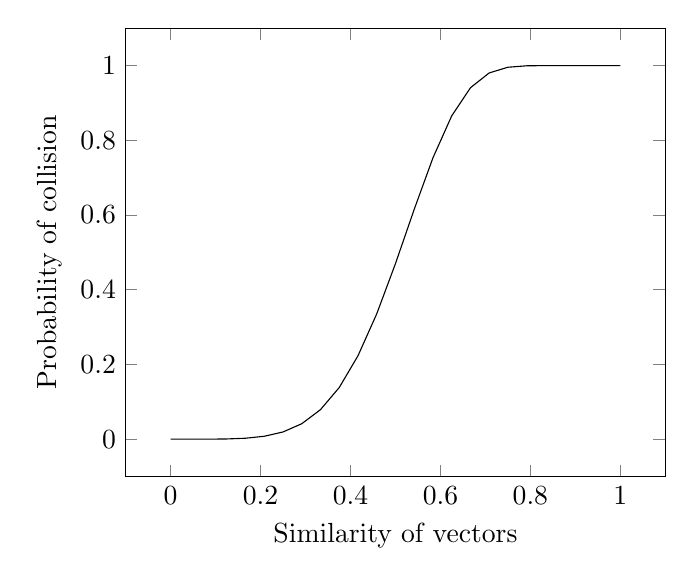
\begin{tikzpicture}
    \begin{axis}[xlabel = {Similarity of vectors}, ylabel = {Probability of collision}]
      \addplot[domain = 0:1]{1 - (1 - x^5)^20};
    \end{axis}
  \end{tikzpicture}

  \caption{The $S$-curve for $s = 5$, $b = 20$}
\end{figure}

\subsection{Covering LSH}
\label{background-covering-lsh}

\textit{To be written}
